\documentclass{article}

\usepackage[T1]{fontenc}    %Schriftart des Dokumentes
\usepackage[ngerman]{babel} %Dokumentensprache, hier Deutsch
\usepackage{amsmath, amssymb, stmaryrd} %mathematische Schriftzeichen
\usepackage{graphicx} %Einfügen von Grafiken
\usepackage{wrapfig}
\usepackage{bm}

\newcommand\myeq{\mathrel{\overset{\makebox[0pt]{\mbox{\normalfont\tiny\sffamily {sin($\phi$)$\approx \phi$}}}}{$\iff$}}}

\setlength{\parindent}{0pt} %Einrückung von Absätzen auf null gesetzt
\setlength{\parskip}{10pt} %Abstand zischen Absätzen auf 10pt gesetzt

\title{Versuch 14: Mathematisches Pendel}
\author{Matthias Kuntz}
\date{21.09.2023}

\begin{document}

\maketitle

%-------------------------EINLEITUNG-------------------------
\section{Einleitung}

In diesem Versuch soll mithilfe eines Fadenpendels die Erdbeschleunigung $g$ bestimmt werden. Dabei wird das Pendel zunächst als theoretisch perfektes mathematisches Pendel betrachtet, anschließend als physikalisches Pendel mit Korrektureffekten wie Reibung und Auftrieb.  

\subsection{Physikalische Grundlagen}

Aus der Schwingdauer $T_0$ sowie der Länge $l$ eines mathematischen Pendels kann direkt die Erdbeschleunigung $g$ ermittelt werden:

\begin{equation}
    \begin{split}
        T_0 &= 2\pi \sqrt{\frac{l}{g}} \\
        g &= 4\pi^2 \frac{l}{T_0^2}
    \end{split}
    \label{eq:1}
\end{equation}

Bei unserem Versuchsaufbau wird die Bestimmung der Länge $l$ der entscheidendste Faktor für die Genauigkeit des Endergebnisses sein. Der Fehler dieser Messung wird deutlich größer sein als der der Schwingungsperiode, da wir die Zeit über viele hunderte Schwingungen messen werden und sich unser Fehler der Zeitmessung eben genau um diese Anzahl als Divisor verringert. Somit kann, wenn wir die Pendellänge mitsamt Fehler bestimmt haben, eine erste Schätzung gemacht werden wie viele Schwingungen wir messen müssen, sodass der Fehler der Schwingungsperiode insignifikant wird. Wir fordern dafür einen Faktor von 0,3 für den relativen Zeitfehler im Vergleich zum Längenfehler. Dazu nutzen wir den Fehler $\Delta g$, der aus Gleichung \ref{eq:1} über die Gauss'sche Fehlerfortpflanzung hervorgeht:

\begin{equation}
    \begin{split}
        \frac{\Delta g}{g} &= \sqrt{\left( \frac{\Delta l}{l} \right)^2 + \left( \frac{2 \Delta t}{n T_0} \right)^2} \\ \\
        \implies \frac{2 \Delta t}{n T_0} &\approx 0,3 \frac{\Delta l}{l}
    \end{split}
    \label{eq:2}
\end{equation}

Wir bekommen so einen Wert für die Zahl $n$, die die Anzahl der Schwingungen darstellt. 

Betrachten wir das Pendel nicht mathematisch sondern physikalisch, so ergibt sich eine Drehschwingung mit Periodendauer

\begin{equation}
    T_D = 2\pi \sqrt{\frac{I}{D}},
    \label{eq:3}
\end{equation}

wobei $I$ das Drehmoment des Pendels und $D$ dessen Winkelrichtgröße darstellt. Wir können das Trägheitsmoment des Pendels als Summe der Trägheitsmomente von Faden und Kugel bestimmen, welche mit dem Steinerschen Satz bestimmt werden. Bei der Drehung um den Aufhängepunkt des Pendels ergibt sich:

\begin{equation}
    \begin{split}
        I_{\text{ges}} &= I_{\text{Kugel}} + I_{\text{Faden}} \\
        &= m_kl^2 + \frac{2}{5}m_k r^2 + \frac{1}{3}m_f l'^2
    \end{split}
    \label{eq:4}
\end{equation}

Hierbei bezeichnent $m_k$ die Masse der Kugel, $m_f$ die des Fadens, $r$ den Radius der Kugel und $l'$ explizit die Länge des Fadens, während $l$ die Gesamtlänge des Pendels darstellt, ergo $l=l'+\frac{1}{2}r$. Lenkt das Pendel nun um einen Winkel $\phi$ aus, so wirkt ein rücktreibendes Drehmoment $M$ abhängig vom Gewicht von Kugel und Faden und verringert um den Auftrieb der Kugel:

\begin{equation}
    \begin{split}
        M &= - \left( (m_k-\rho_L V_k)g \sin{(\phi)l + \frac{1}{2} m_fg \sin{(\phi)}l'} \right)
    \end{split}
    \label{eq:5}
\end{equation}

Hierbei sind $\rho_L$ als Dichte der Luft und $V_k$ als Volumen der Kugel die relevanten Größen für den Auftrieb. Mit der Kleinwinkelnäherung sin($\phi$)$\approx \phi$ und der Dichte der Kugel $\rho_k =m_kV_k$ ergibt sich:

\begin{equation}
    \begin{split}
        M &= - \left( m_k \left( 1 - \frac{\rho_L}{\rho_k} \right) + \frac{1}{2} m_f \right) gl \phi
    \end{split}
    \label{eq:6}
\end{equation}

Mit $D=-\frac{M}{\phi}$ kann man $D$ in Gleichung \ref{eq:3} einsetzen und mit ersten Näherungen erhält man die Form

\begin{equation}
    T_1^2 = 4\pi^2 \frac{l}{g} \left( 1+\frac{2}{5}\frac{r^2}{l^2}+\frac{\rho_L}{\rho_k}-\frac{1}{6}\frac{m_f}{m_k} \right),
\end{equation}

woraus man unter Berücksichtigung der Abhängigkeit der Schwingungsdauer vom Winkelausschlag $\phi_0$ sowie dem Einfluss der Dämpfung $\delta$ die folgende finale Form erhält:

\begin{equation}
    T_g^2 = 4\pi^2 \frac{l}{g} \left( 1+\frac{2}{5}\frac{r^2}{l^2}+\frac{\rho_L}{\rho_k}-\frac{1}{6}\frac{m_f}{m_k}+\frac{\delta^2}{\omega_0^2}+\frac{\phi_0^2}{8} \right)
    \label{eq:8}
\end{equation}

Im Kontext unseres Versuchs ist $T_g$ die gemessene Periodendauer. Die Dämpfung $\delta$ kann über die zeitliche Abnahme der Amplitude, gegeben durch

\begin{equation}
    a(t) = a_0 e^{-\delta t},
 \end{equation}

ermittelt werden.

\subsection{Versuchsaufbau}

Der Versuchsaufbau besteht aus einer Eisenkugel, die an einem dünnen Eisenfaden hängt, der an einem Stativ frei hängend angebracht ist. Am Stativ ist eine Schiene mit Spiegelskala, die das Ablesen der Höhe der Pendelaufhängung ermöglicht. Zusätzlich ist etwa auf Höhe der Kugel eine horizontale Spiegelskala zum Ablesen der Auslenkung des Pendels angebracht. Unter der Kugel wird eine Lichtschranke mit Zähler angebracht und auf einem Display angezeigt, wie oft die Kugel schon vorbeigeschwungen ist. Ziel des Experiments ist es, bei einer langen Schwingung von mehreren hundert Perioden in regelmäßigen Periodenintervallen die Amplitude und Zeit zu messen, um in der Auswertung die Erdbeschleunigung zu bestimmen. 

%---------------VERSUCHSPROTOKOLL MIT MESSDATEN---------------
\newpage

\section{Versuchsprotokoll mit Messdaten}

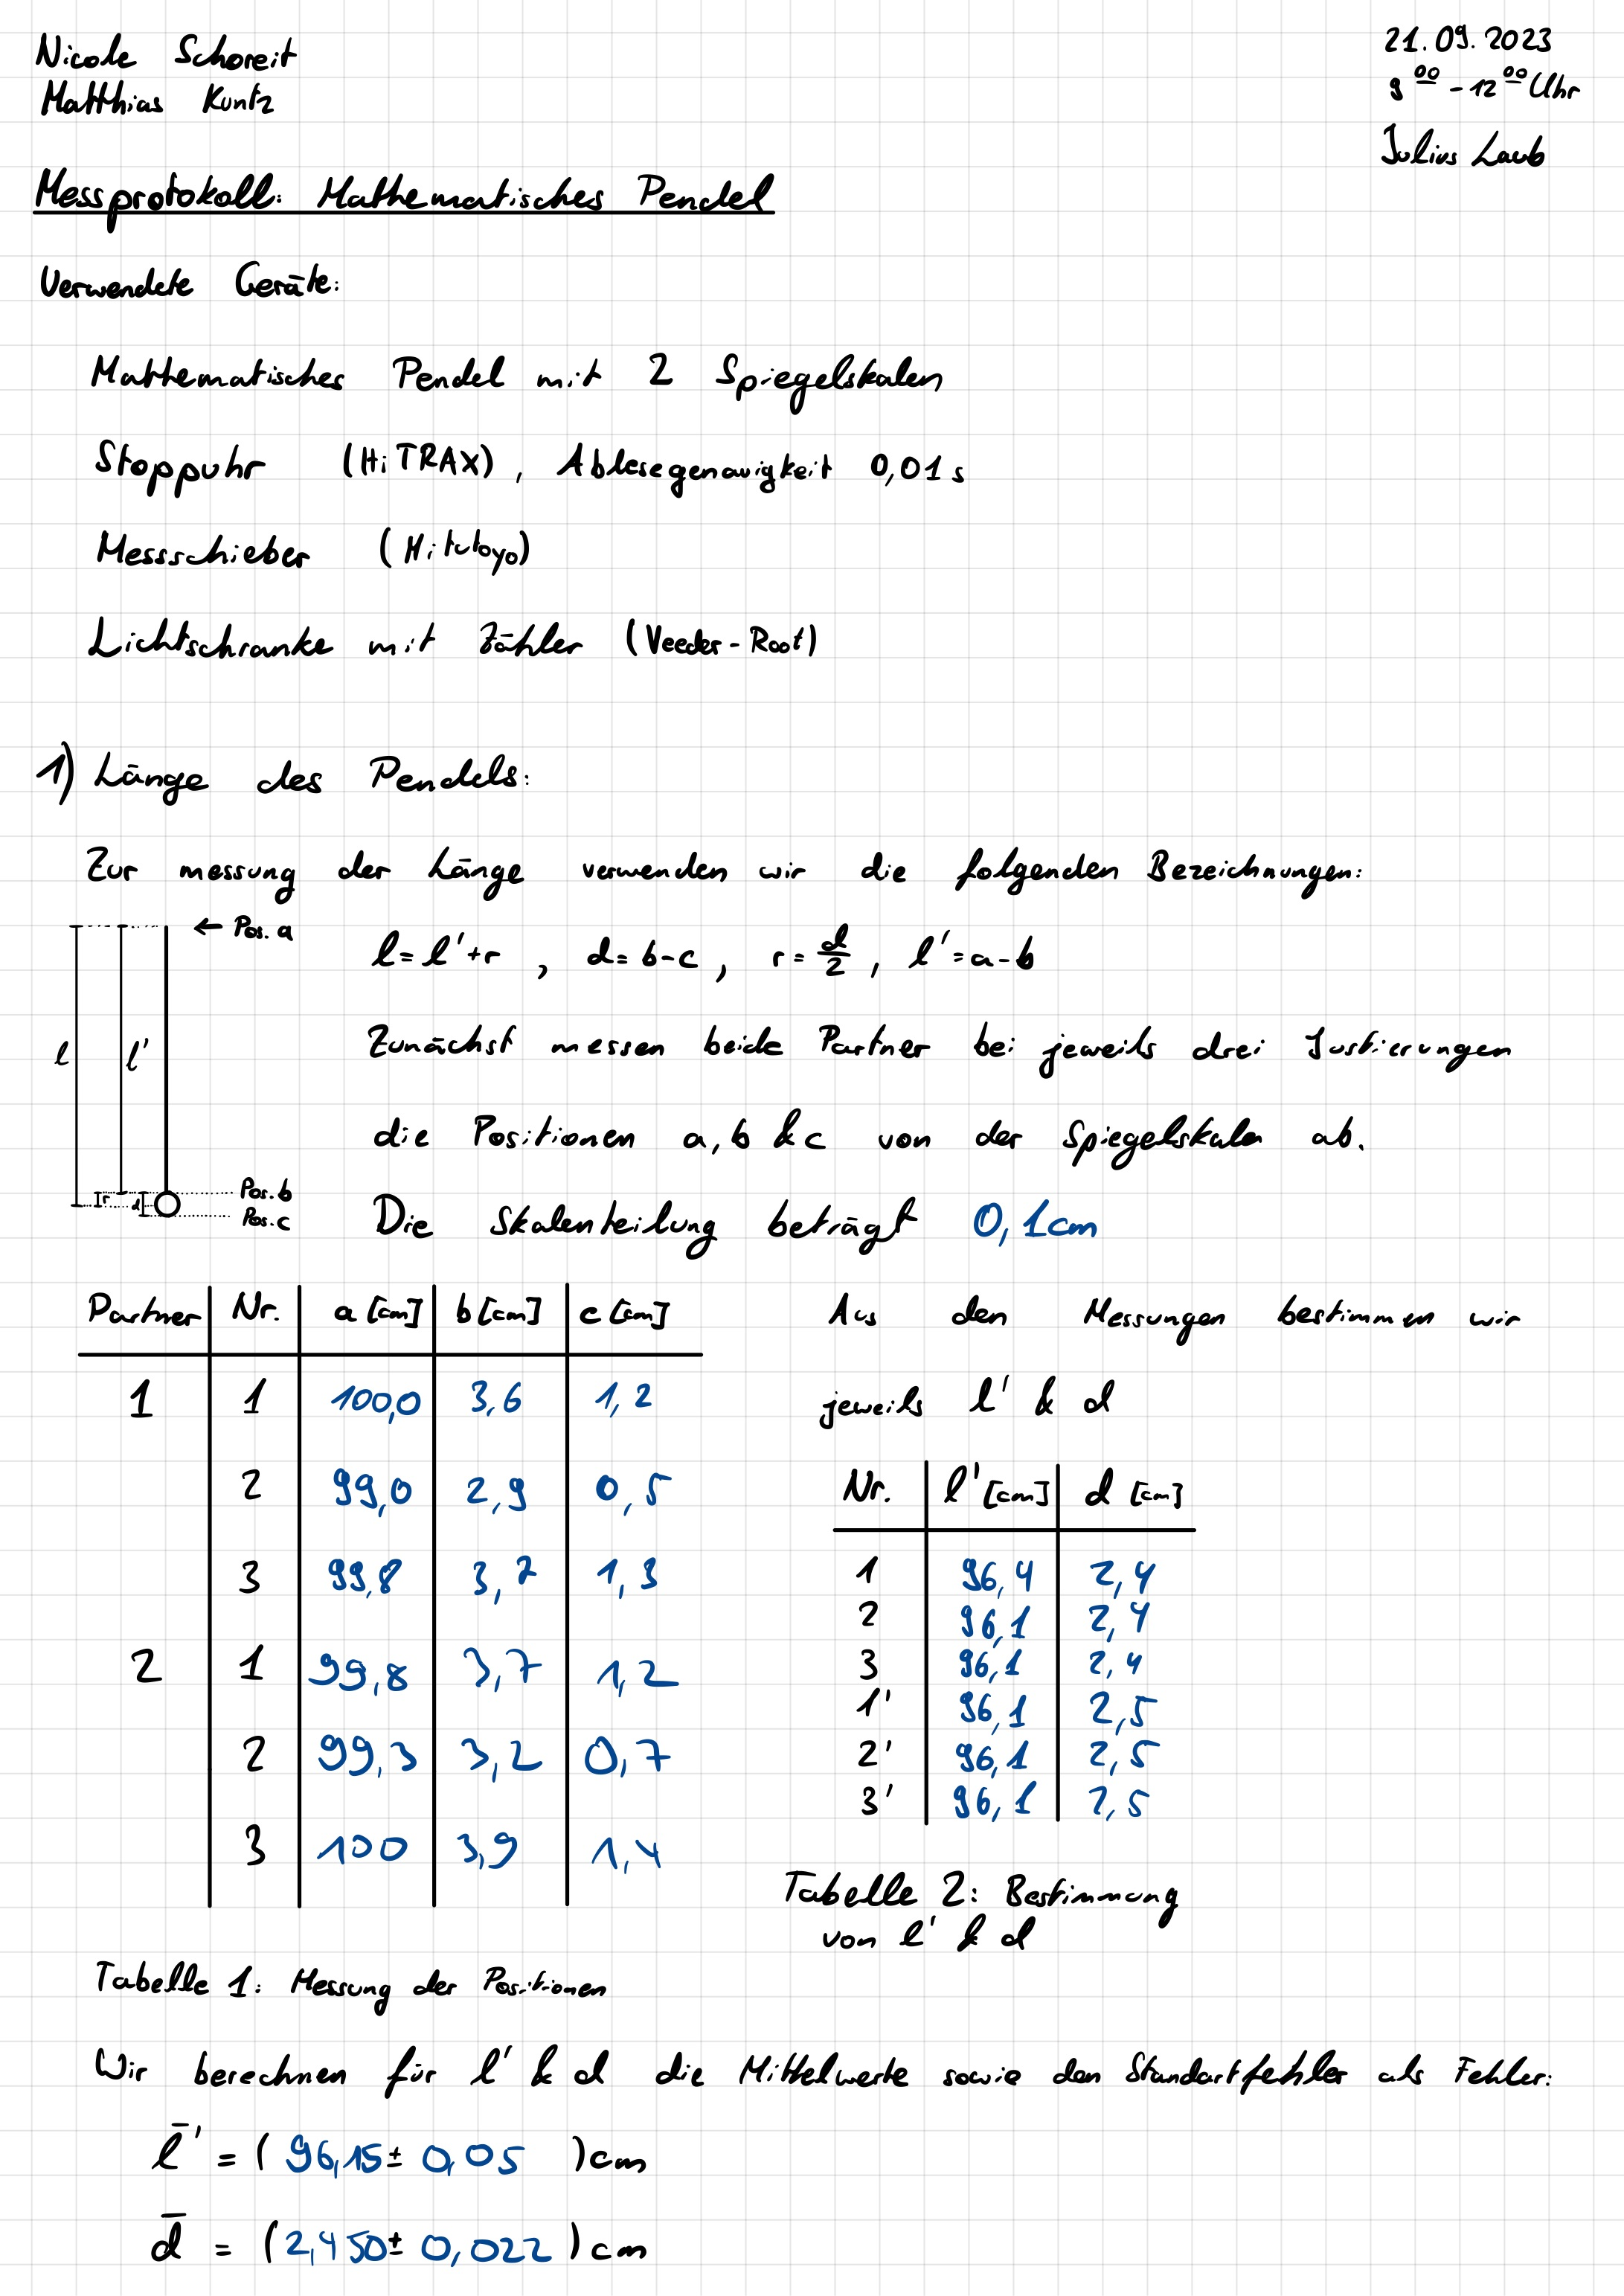
\includegraphics[width=\textwidth]{graphics/mess1.jpg}
\newpage
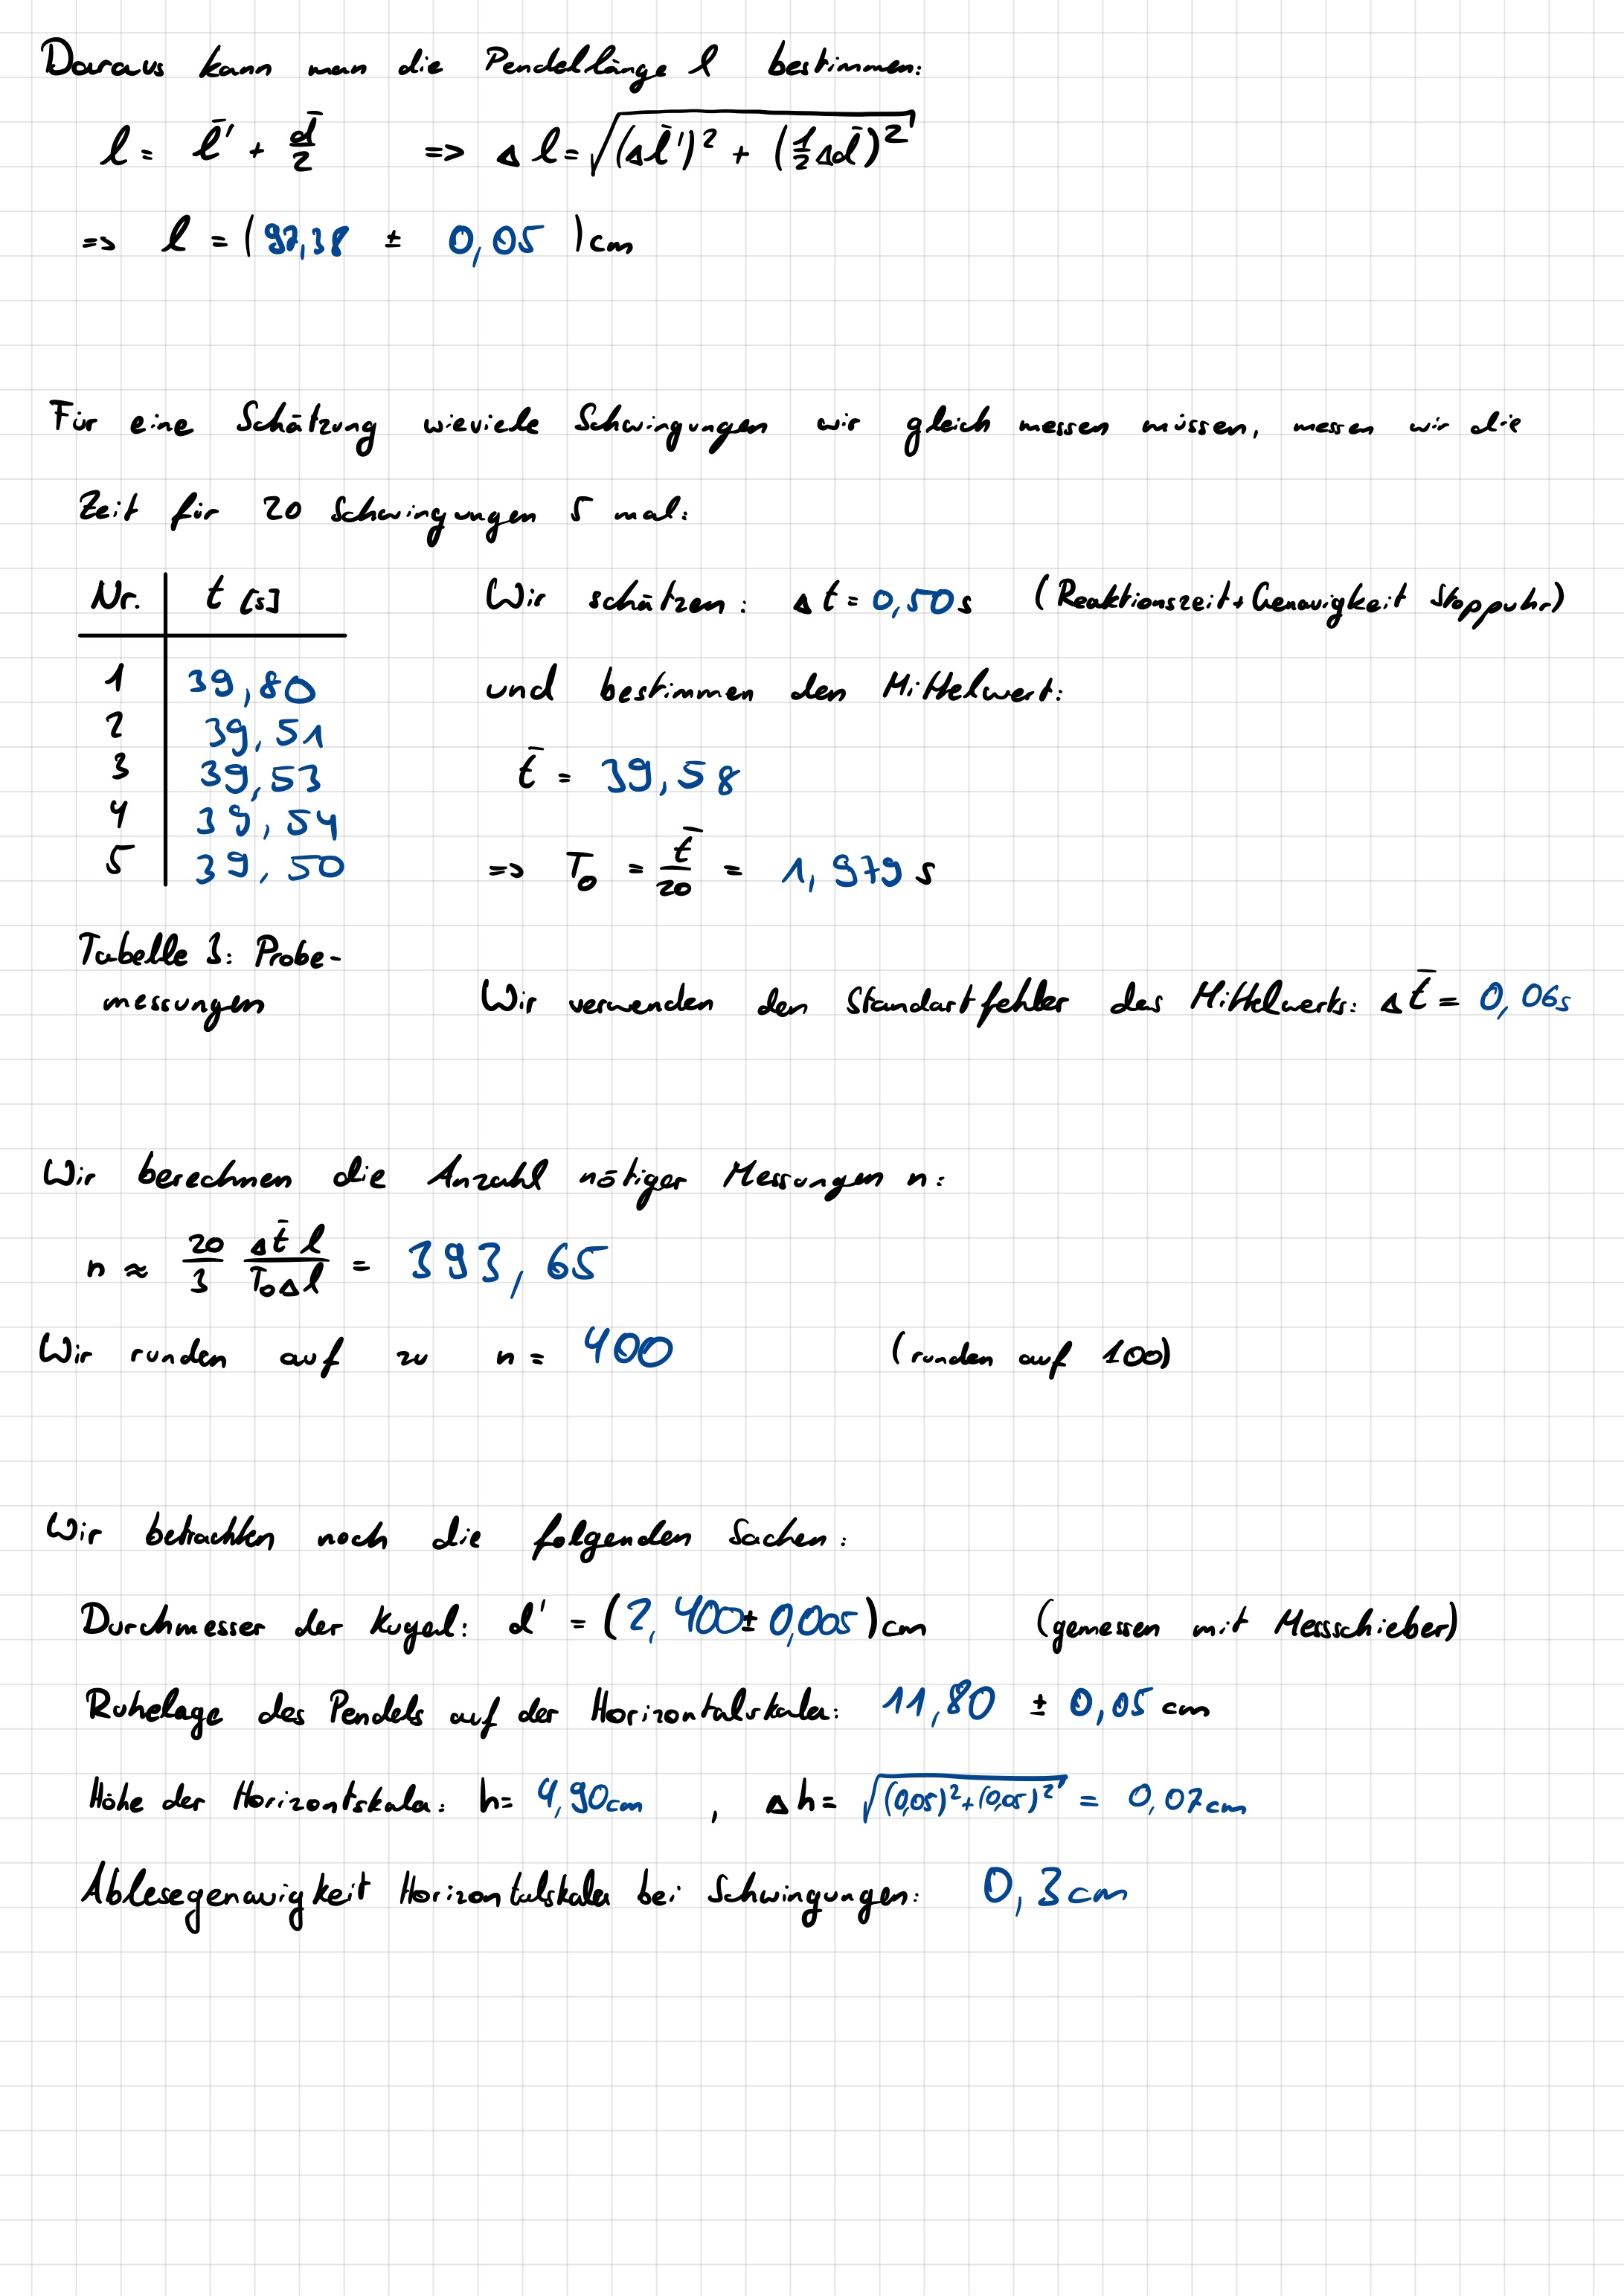
\includegraphics[width=\textwidth]{graphics/mess2.jpg}
\newpage
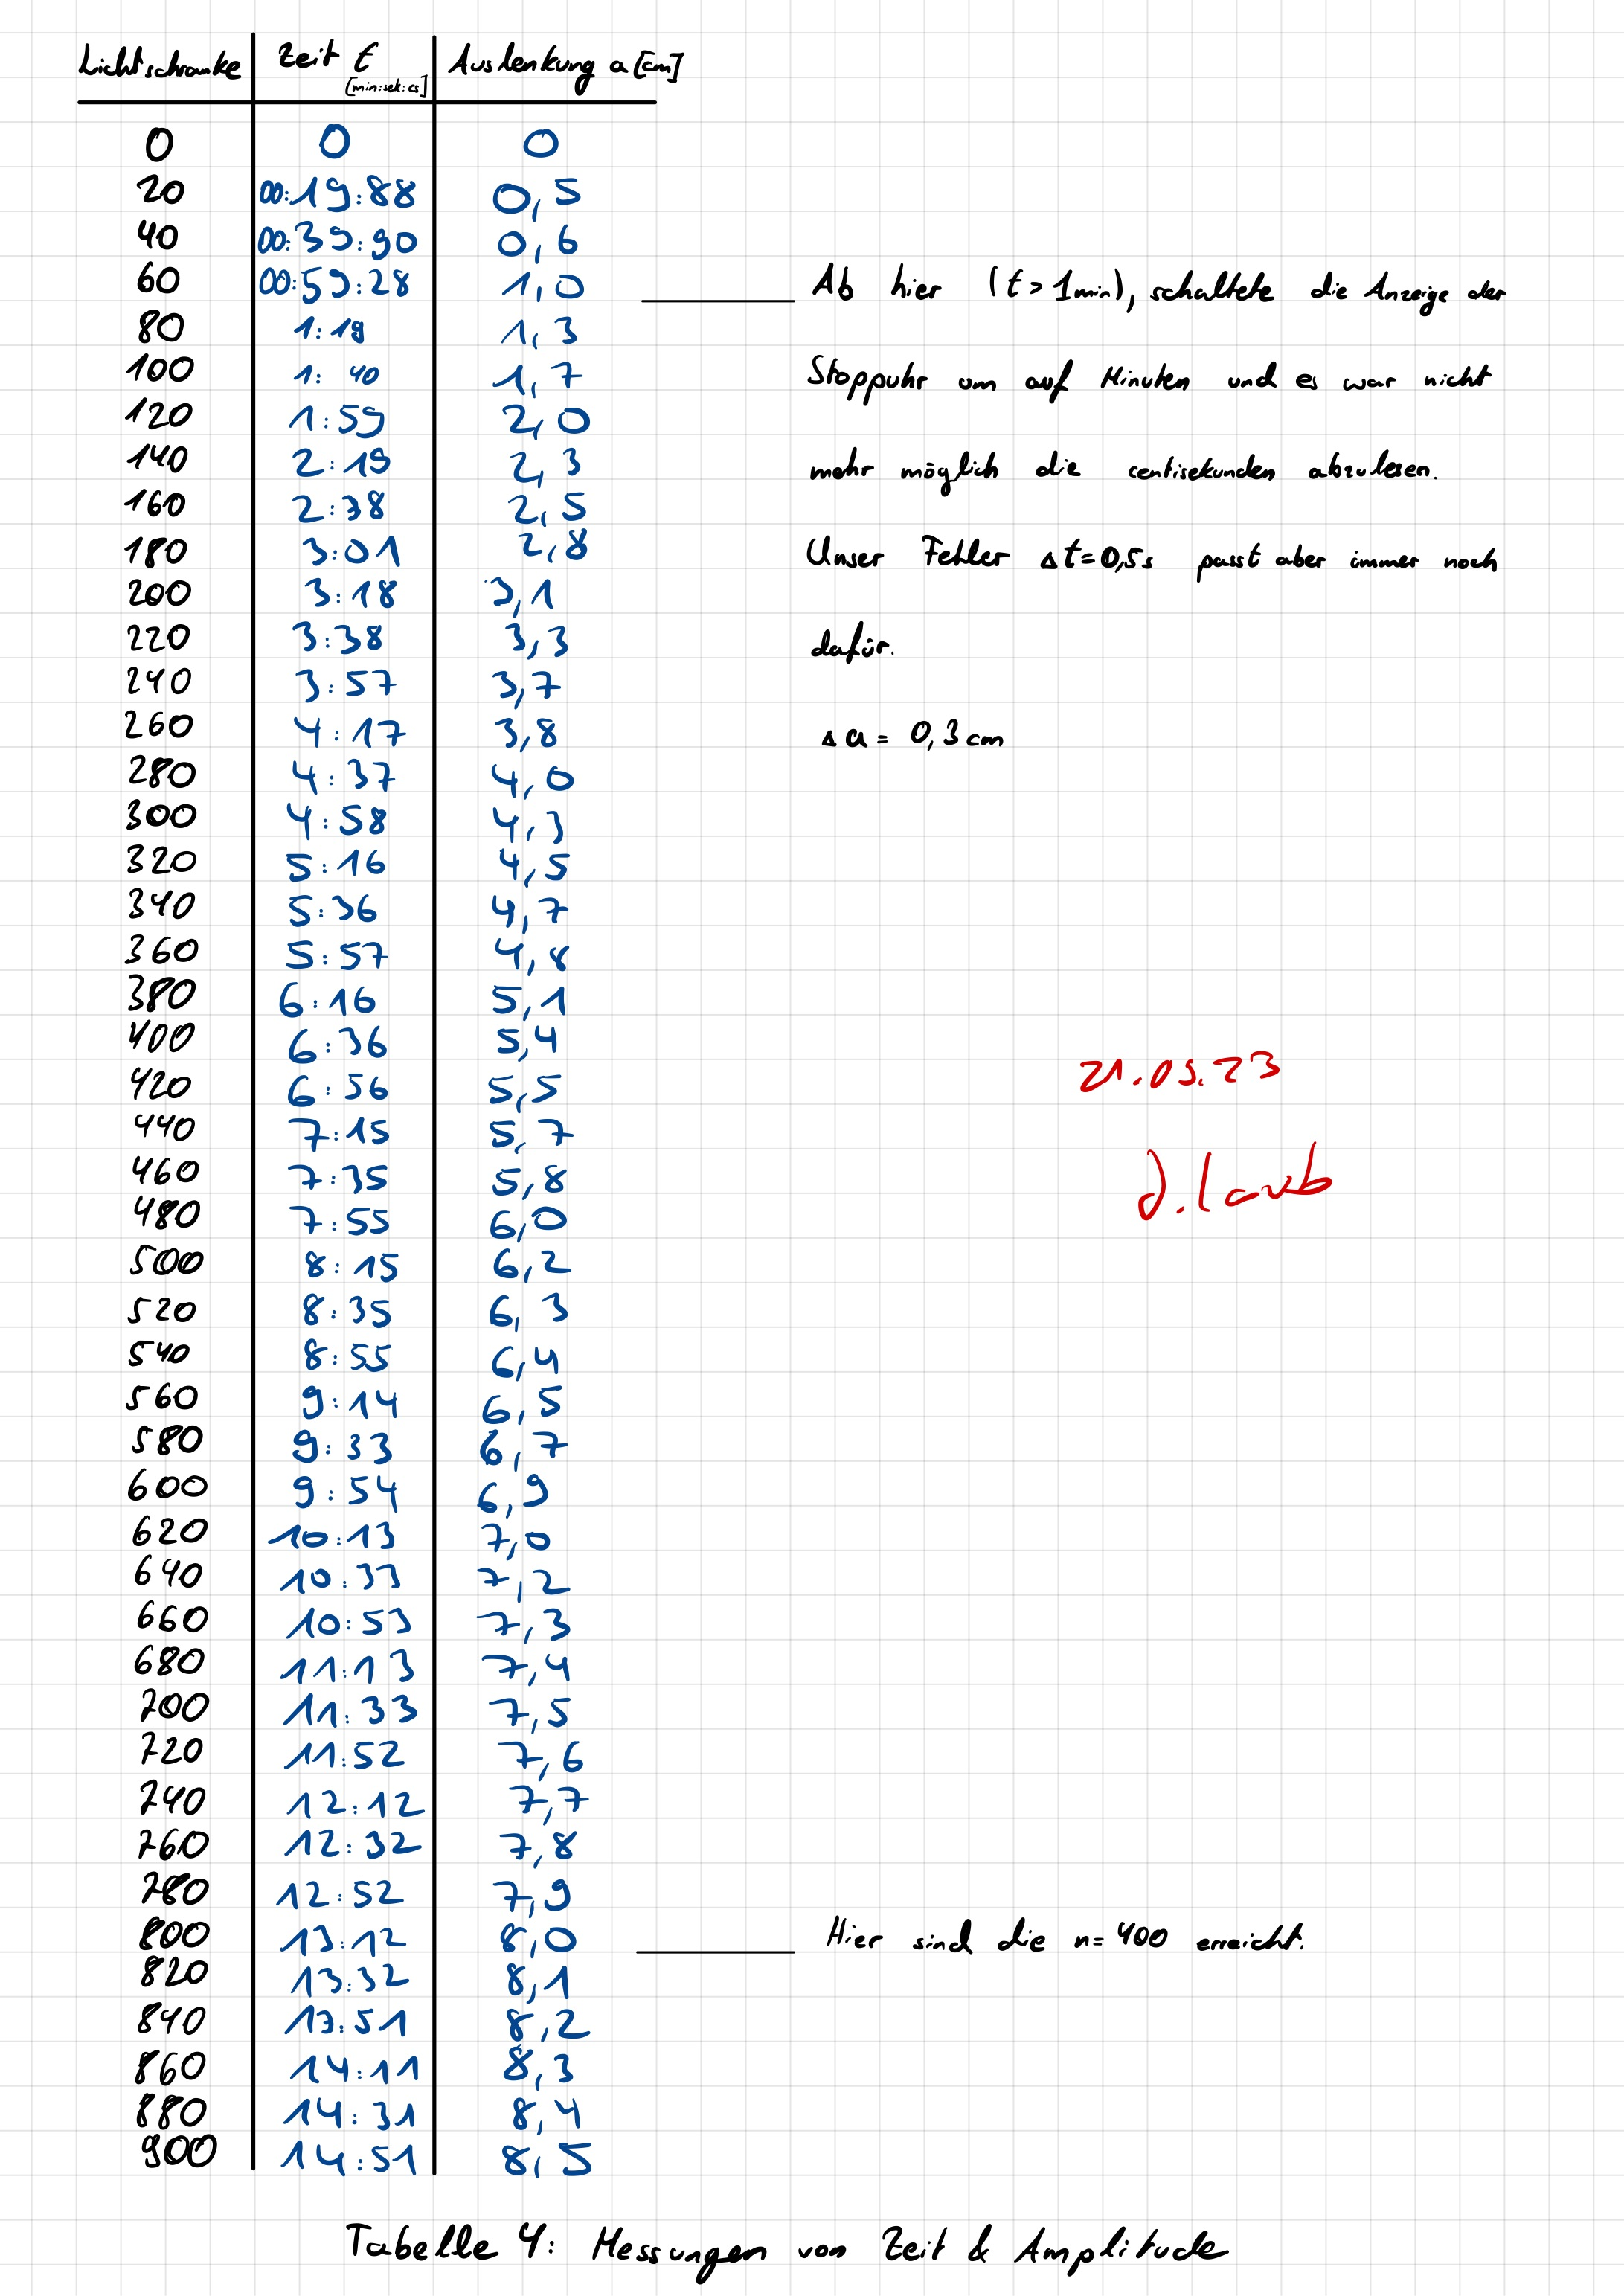
\includegraphics[width=\textwidth]{graphics/mess3.jpg}
\newpage

\addtocounter{table}{4}

%-------------------------AUSWERTUNG-------------------------
\section{Auswertung}

In dieser Evaluation werden alle Fehler, sofern keine spezifische Angabe gemacht wird, mithilfe der Gauss'schen Fehlerfortpflanzung berechnet. Dies bedeutet, dass ein Wert $F$, der mit der Formel $f(a_1, ..., a_n)$ berechnet wird, den Fehler $\Delta F$ gegeben über folgende Formel hat:

\begin{equation}
    \Delta F = \sqrt{\sum_n \left( \frac{\partial f}{\partial a_n} \cdot \Delta a_n \right)^2}.
\end{equation}

\subsection{Fallbeschleunigung ohne Korrektureffekte}

Wir beginnen indem wir aus der gemessenen Zeit in Tabelle 4 die Periodendauer $T$ einer Schwingung berechnen. Dazu nehmen wir den zuletzt gemessenen Wert für die Zeit $t_{max}=891$s und teilen diesen durch die Anzahl $n$ (hier $n=450$, da der Zähler doppelt pro Oszillation zählt):

\begin{equation}
    \begin{split}
        T &= \frac{t_{max}}{n},  \ \  \ \ \Delta T = \frac{\Delta t_{max}}{n} \\ \\
        T &= (1,9800 \pm 0,0011) \text{s} \\
    \end{split}
\end{equation}

Zusammen mit der im Messprotokoll ermittelten Pendellänge $l$ können wir nun über Gleichung \ref{eq:1} die Erdbeschleunigung $g$ bestimmen:

\begin{equation}
    \begin{split}
        g = 4\pi^2 \frac{l}{T^2}, \ \ & \ \ \Delta g = \frac{4 \pi^2}{T^2} \sqrt{\left( \Delta l \right)^2 + \left( \frac{l}{T} \cdot \Delta T \right)^2} \\ \\
        \bm{g} &= \bm{(9,806 \pm 0,015) \frac{\textbf{m}}{\textbf{s}^2}}
    \end{split}
\end{equation}

Wir vergleichen diesen Wert mit dem im Skript gegeben Heidelberger Standard-Wert von $g_{HD} = (9,80984 \pm 0,00002) \frac{\text{m}}{\text{s}^2}$ :

\begin{equation}
    \begin{split}
        \sigma = \frac{|g-g_{HD}|}{\sqrt{(\Delta g)^2+(\Delta g_{HD})^2}} = 0,26
    \end{split}
\end{equation}

\subsection{Fallbeschleunigung mit Korrektureffekten}

Zunächst tragen wir die gemessene Amplitude als Funktion der Zeit auf eindekadisches Logarithmenpapier auf. Dafür verrechnen wir zunächst die Messwerte der Amplitude mit dem Wert in Ruhelage, um auf die eigentliche Amplitude zu kommen. Das Diagramm ist in Abbildung \ref{fig:dämpfung} zu sehen. Wir ermitteln über die Steigung $m$, gegeben durch

\begin{equation}
    \begin{split}
        m &= \frac{\Delta a}{\Delta t} \\
        \Delta m &= \left| m - \frac{\Delta a_f}{\Delta t_f} \right| \\ \\
        m &= (0,64 \pm 0,03) \cdot 10^{-3} \frac{1}{\text{s}}
    \end{split}
    \label{res:m}
\end{equation}

die Dämpfung $\delta$:

\begin{equation}
    \begin{split}
        \delta &= \frac{m}{\log{e}}, \ \ \ \Delta \delta = \frac{\Delta m}{\log{e}} \\ \\
        \delta &= (1,48 \pm 0,07) \cdot 10^{-3} \frac{1}{\text{s}}
    \end{split}
    \label{res:delta}
\end{equation}

Zusätzlich berechnen wir das Verhältnis der Masse des Fadens $m_f$ und der der Kugel $m_k$

\begin{equation}
    \begin{split}
        \frac{m_f}{m_k} &= \frac{\pi \left( \frac{d_f}{2} \right)^2 l' \rho_{Eisen}}{\frac{4}{3}\pi \left( \frac{d_k}{2} \right)^3 \rho_{Eisen}} = l' \frac{3}{2} \frac{d_f^2}{d_k^3} \\
        \Delta \frac{m_f}{m_k} &= \frac{m_f}{m_k} \sqrt{\left( \frac{\Delta l'}{l'} \right)^2 + \left( \frac{\Delta d_k}{d_k} \right)^2} \\ \\
        \frac{m_f}{m_k} &= (3,92 \pm 0,04) \cdot 10^{-3}
    \end{split}
    \label{res:masses}
\end{equation}

\newpage

sowie die Kreisfrequenz $\omega_0$ des Pendels:

\begin{equation}
    \begin{split}
        \omega_0 &= \frac{2\pi}{T} \\
        \Delta \omega_0 &= \frac{2\pi}{T^2}\cdot \Delta T \\ \\
        \omega_0 &= (3,1733 \pm 0,0018) \text{Hz}
    \end{split}
    \label{res:omega}
\end{equation}

Zuletzt werden noch die durchschnittliche Schwingungsdauer $\overline{a}$ und daraus $\phi_0$ bestimmt, wobei wieder $t_{max}=891$s und $a_0 = 11,8$cm gilt:

\begin{equation}
    \begin{split}
        \overline{a} &= \frac{\int_0^{t_{max}} a_0 e^{-\delta t}dt}{t_{max}} \\ \\
        \phi_0 &= \arctan{\frac{\overline{a}}{l}} = 0,0655 \text{rad}
    \end{split}
    \label{res:phi0}
\end{equation}

Die Berücksichtigung des Fehlers wurde hierbei ausgelassen, da dieser im Vergleich zum bestimmten Wert vernachlässigbar klein ist.

Nun können wir anhand Gleichung \ref{eq:8} die korrigierte Erdbeschleunigung $g'$ bestimmen. Dabei ist anzumerken, dass im Fehler der mit $K$ bezeichnete Term für den Gesamtfehler der ganzen Korrekturterme steht. Dieser ist, da nach Abschätzungen festgestellt wurde, dass er die Größenordnung $10^{-6}$ hat und somit von den anderen Fehlern um $10^4$ Größenordnungen übertroffen wird, hier nicht beachtenswert und würde sowieso keinen Einfluss auf die signifikanten Stellen des Fehlers nehmen:

\begin{equation}
    \begin{split}
        g' &= 4\pi^2 \frac{l}{T_g^2} \left( 1+\frac{2}{5}\frac{r^2}{l^2}+\frac{\rho_L}{\rho_k}-\frac{1}{6}\frac{m_f}{m_k}+\frac{\delta^2}{\omega_0^2}+\frac{\phi_0^2}{8} \right) \\
        \Delta g' &= g \sqrt{\left( \frac{\Delta l}{l} \right)^2 + \left( \frac{2 \Delta T_g}{T_g} \right)^2 + \left( \frac{\Delta K}{K} \right)^2} \\ \\
        \bm{g'} &= \bm{(9,807 \pm 0,012) \frac{\textbf{m}}{\textbf{s}^2}}
    \end{split}
\end{equation}

Vergleicht man dieses Ergebnis nun wieder über die Sigmaabweichung mit dem Heidelberger Standard-Wert so erhält man:

\begin{equation}
    \sigma' = 0,23
\end{equation}

Man erkennt, dass die Abweichung vom physikalischen $g'$ kleiner ist als die vom mathematischen $g$.

\bigskip

\bigskip

\bigskip

\begin{figure} [!h]
    \centering
    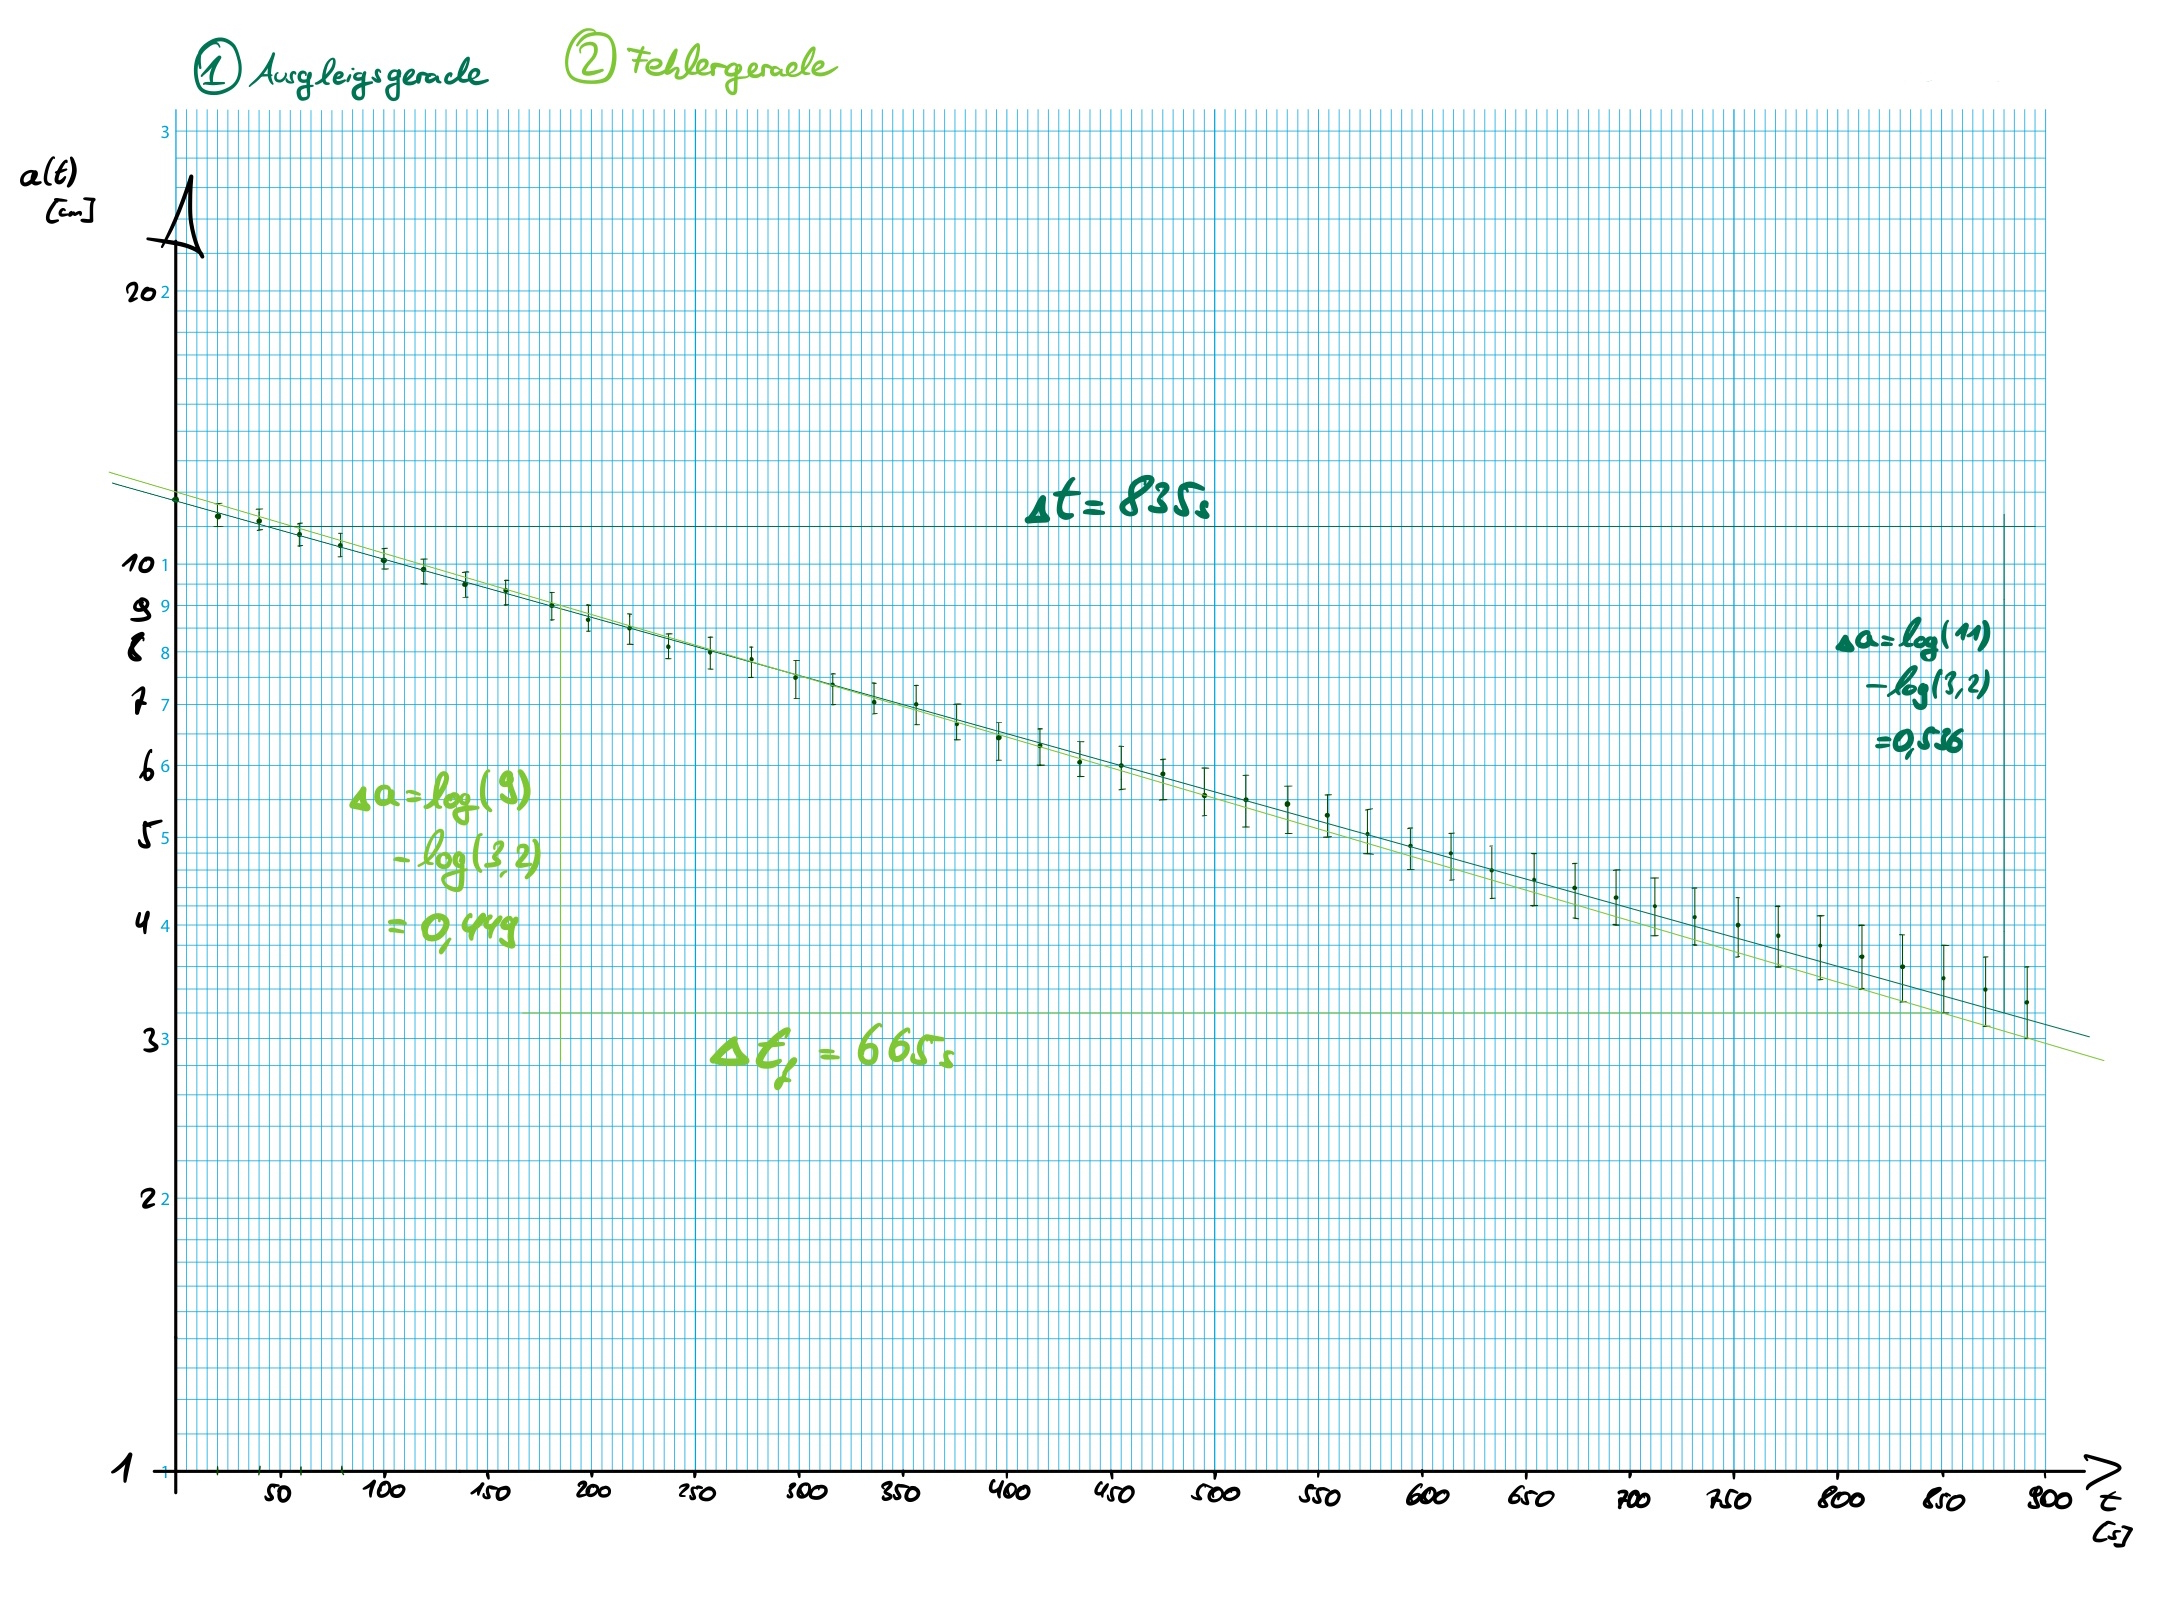
\includegraphics[width=\textwidth]{graphics/dia1.jpg}
    \caption{Bestimmung der Steigung für die Dämpfung}
    \label{fig:dämpfung}
\end{figure}

\newpage
%---------------PRÄSENTATION DER ENDERGEBNISSE---------------
\section{Präsentation der Endergebnisse}

In diesem Versuch wurde mit zwei verschiedenen Betrachtungsweisen die Erdbeschleunigung bestimmt. Zunächst betrachteten wir unsere Messwerte so, als kämen sie von einem perfekten mathematischen Pendel und bekamen  

\begin{equation}
    \bm{g} = \bm{(9,806 \pm 0,015) \frac{\textbf{m}}{\textbf{s}^2}}.
\end{equation}

Anschließend berüchtigten wir Korrektureffekte und betrachteten somit das physikalische Pendel. Hier erhielten wir den Wert

\begin{equation}
    \bm{g'} = \bm{(9,807 \pm 0,012) \frac{\textbf{m}}{\textbf{s}^2}}.
\end{equation}


\newpage
%---------------ZUSAMMENFASSUNG UND DISKUSSION---------------
\section{Zusammenfassung und Diskussion}

In diesem Versuch wurde mithilfe eines Pendels die Erdbeschleunigung bestimmt, einmal mit und einmal ohne Korrektureffekte.

Zunächst lässt sich positiv vermerken, dass beide Ergebnisse innerhalb erwarteter Bereiche und innerhalb insignifikanter Abweichungen vom Literaturwert blieben. Beide bestimmten Werte für die Erdbeschleunigung lagen mit Sigmaabweichungen von $\sigma = 0,26$ und $\sigma' = 0,23$ sehr gut innerhalb der 1$\sigma$-Intervalle und das obwohl die Fehler sogar relativ nur bei 0,15 und 0,12 Prozent des jeweiligen Endwerts lagen. Es ist auch zu vermerken, dass der zweite Wert nicht nur näher beim Literaturwert liegt, sondern auch den kleineren Fehler aufweist. Somit lassen sich im Kontext des Versuchsaufbaus nur minimale Verbesserungsmöglichkeiten finden. 

Wie in der Einführung bereits erwähnt wird die Genauigkeit des Endergebnisses zum Großteil von der Genauigkeit der Längenmessung des Pendels bestimmt. Hier wurden zwar durch die Verwendung des sehr genauen Messschiebers und der fünffachen Wiederholung der Längenmessung eine recht hohe Präzision erzielt, jedoch fiel während des Experimentierens auf, dass beispielsweise der Faden durch das recht geringe Gewicht unserer kleinen Kugel nicht immer ganz gespannt war uns sich besonders an der Aufhängung oben und der Verbindung zur Kugel unten leicht beugte. Auch ist der Aufhängungspunkt selbst immer eine potenzielle Fehlerquelle für leichte Höhenvariationen. 

Die wohl größten Ungenauigkeiten gab es aber beim Bestimmen der Amplitude. Hier war es besonders schwierig, immer alle paar Perioden die Position des schwingenden Pendels zu bestimmen, weshalb auch der vergleichsweise hohe Fehler von 0,3cm abgeschätzt wurde. Weitergehend ist natürlich auch nicht klar, ob diese Abschätzung überhaupt ausreichend war. Eine Verbesserung könnte hier zum Beispiel durch das Aufzeichnen der Schwingungen mit einer Kamera und die nachfolgende Auswertung anhand des verlangsamten Videos liefern. Dabei wäre es nur bei einer Gesamtschwingdauer von etwa 15 Minuten recht aufwendig den Überblick zu behalten.  

Zuletzt lässt sich noch kurz die Ungenauigkeit des grafischen Verfahrens nennen. Manuell per Hand Punkte einzeichnen, Ausgleichsgeraden finden und Fehlergeraden abschätzen ist nämlich immer etwas ungenau. Computerbasierte Visualisierungen hätten hier ein genaueres Ergebnis liefern können.


Zusammenfassen lässt sich sagen, dass trotz der genannten potenziellen Fehlerquellen durch die Kombination der sehr geringen Sigmaabweichungen und den relativ gesehen kleinen Fehlern ein  zufriedenstellendes Endresultat erzielt werden konnte.

\end{document}
